%
%  愛知工業大学 情報科学部 情報科学科
%    要旨集用LaTeXテンプレート(2016.11.28)
%
%  original by Nobuhiro Ito
%  revised by Susumu Suzuki & Masashi Morimoto on 2016.11.28
%
\documentclass{jarticle}
\pagestyle{empty}

%% レイアウト
\setlength{\topmargin}{-10.4mm}
\setlength{\headheight}{0mm}
\setlength{\headsep}{0mm}
\setlength{\textheight}{262mm}
\setlength{\textwidth}{180mm}
%\setlength{\topskip}{7mm}
\setlength{\evensidemargin}{-10.4mm} 
\setlength{\oddsidemargin}{-10.4mm} 
\setlength{\columnsep}{8mm}

%% パッケージ環境
% graphicx: 画像読み込み
%  dvipdfmxをドライバ指定することでpdf/png/jpeg形式の図を利用可能
%  異なるドライバを利用する場合はそのドライバ指定に変更
% \usepackage{graphicx} % suzuki
\usepackage[dvipdfmx]{graphicx} % suzuki
% subcaption: subfigureを置き換えたパッケージ(複数の図用)
% \setlength{\footskip}{12mm}
% \usepackage{subfigure}	 % suzuki
\usepackage{subcaption} % suzuki
% color:文章に色をつけたいとき
%  利用例:\textcolor{red}{文章}
% \usepackage{color}
\usepackage{booktabs}
\usepackage{setspace}

% 行間調整
\setstretch{0.9}

%sectionのフォントサイズ修正
\makeatletter
\def\section{\@startsection {section}{1}{\z@}{2.5ex plus -1ex minus -.2ex}{1.3 ex plus .1ex}{\large\bf}}
\makeatother 

%subsectionのフォントサイズ修正
\makeatletter
\def\subsection{\@startsection {subsection}{1}{\z@}{1.5ex plus -1ex minus -.4ex}{0.3 ex plus .1ex}{\bf}}
\makeatother 

\begin{document}
\twocolumn[

\begin{center}
%タイトル
{\LARGE \textbf{要旨集の書き方&テンプレート}}\\
%サブタイトル
%{\Large \textbf{必要に応じてサブタイトル}}
\end{center}

\begin{center}
% 著者
\begin{tabular}{cccc}
% 1名の場合
%\multicolumn{4}{c}{K11001 愛工総和}\\
% 2名の場合
%& K11002 愛工七音 & X11003 愛工頼音 &\\
% 3名の場合
%K11001 愛工総和 & K11002 愛工今鹿 & X11003 愛工姫星&\\
% 4名の場合
K11001 愛工総和 & K11002 愛工今鹿 & X11003 愛工姫星& X11004 愛工緑輝\\
% 指導教員
\multicolumn{4}{c}{\textbf{指導教員} 愛工一郎}
\end{tabular}
\hspace{2zw}
\end{center}
]

%--------------------------------------------
\section{はじめに}
\label{sec:intro}
これは卒業論文・卒業制作要旨集の p\LaTeX2e 用テンプレートである.
伊藤暢浩先生が作ったテンプレートをベースに,sectionとsubsectionのフォントサイズ変更,カラム間のマージン変更などを施している.
なお,書式が同じであればWordやPagesを使っても構わない.

%--------------------------------------------
\section{レジュメの構成について}
\label{sec:const}

要旨集(レジュメ)のタイトル(及びサブタイトル)は卒業論文のタイトルと一致していなくてはならない.

レジュメの節(section)構成は様々なものが考えられ,研究内容や制作内容によっても異なるが,一般的には研究背景,目的および研究概要を記述する「{\bf はじめに}」で始まる.
そして研究全体のまとめ,結論,今後の課題を記述する「{\bf まとめ}」や「{\bf むすび}」で締めくくる.
全体的には5$\sim$6個の節で構成され,必要に応じて小節(subsection)を用いる.

%--------------------------------------------
\section{記述する文章について}
\label{sec:description}

\emph{研究の内容や記述する文章はオリジナルである必要がある.単に他の研究や実験を流用したり,インターネットや他の文献などの文章をそのままコピーして使用したりすることなどは決してあってはならない.レジュメは大量に印刷されて多くの人が読むため,コピーした文章の使用はすぐに誰かが見つける.} % changed to \emph by morimoto


%--------------------------------------------
\section{図や表について}
\label{sec:figure}

必要に応じて図や表を用いる.
使用した図や表についてはキャプションを付けるとともに,必ず本文中で図表番号を参照する.

\emph{図や表は自分で作成したものを使用する.標準テストイメージ等を除き,インターネット等で入手した図や写真,表などをそのまま使ってはならない.} % changed to \emph by morimoto

% revised by morimoto
レジュメは基本的にモノクロで印刷されるが,必要に応じてカラーの図や画像を用いることができる.
またオフセット印刷で製本するため,十分に鮮明な図や画像を用意しておくとよい.

% revised by suzuki & morimoto (from EPS to PDF)
\LaTeX の場合,図のファイルはPDF形式で用意することが推奨されている\cite{tex}.
また,EPS形式を用いることができる.
Illustratorなどのソフトで作成して,保存するときに\LaTeX で使用可能な画像形式を指定すればよい.
%
PNG形式やJPEG形式を用いることもできるが,場合によっては図の外枠を明示的に指定する必要がある.

図 \ref{fig:1}は,単独の図である.
また図 \ref{fig:2}は複数で構成される図である.
またfigure*環境を用いることで1カラムの図を使用することも可能である.
%
また,表のサンプルを表 \ref{tab:sample}に示す.

\begin{figure}[htb]
\centering
% 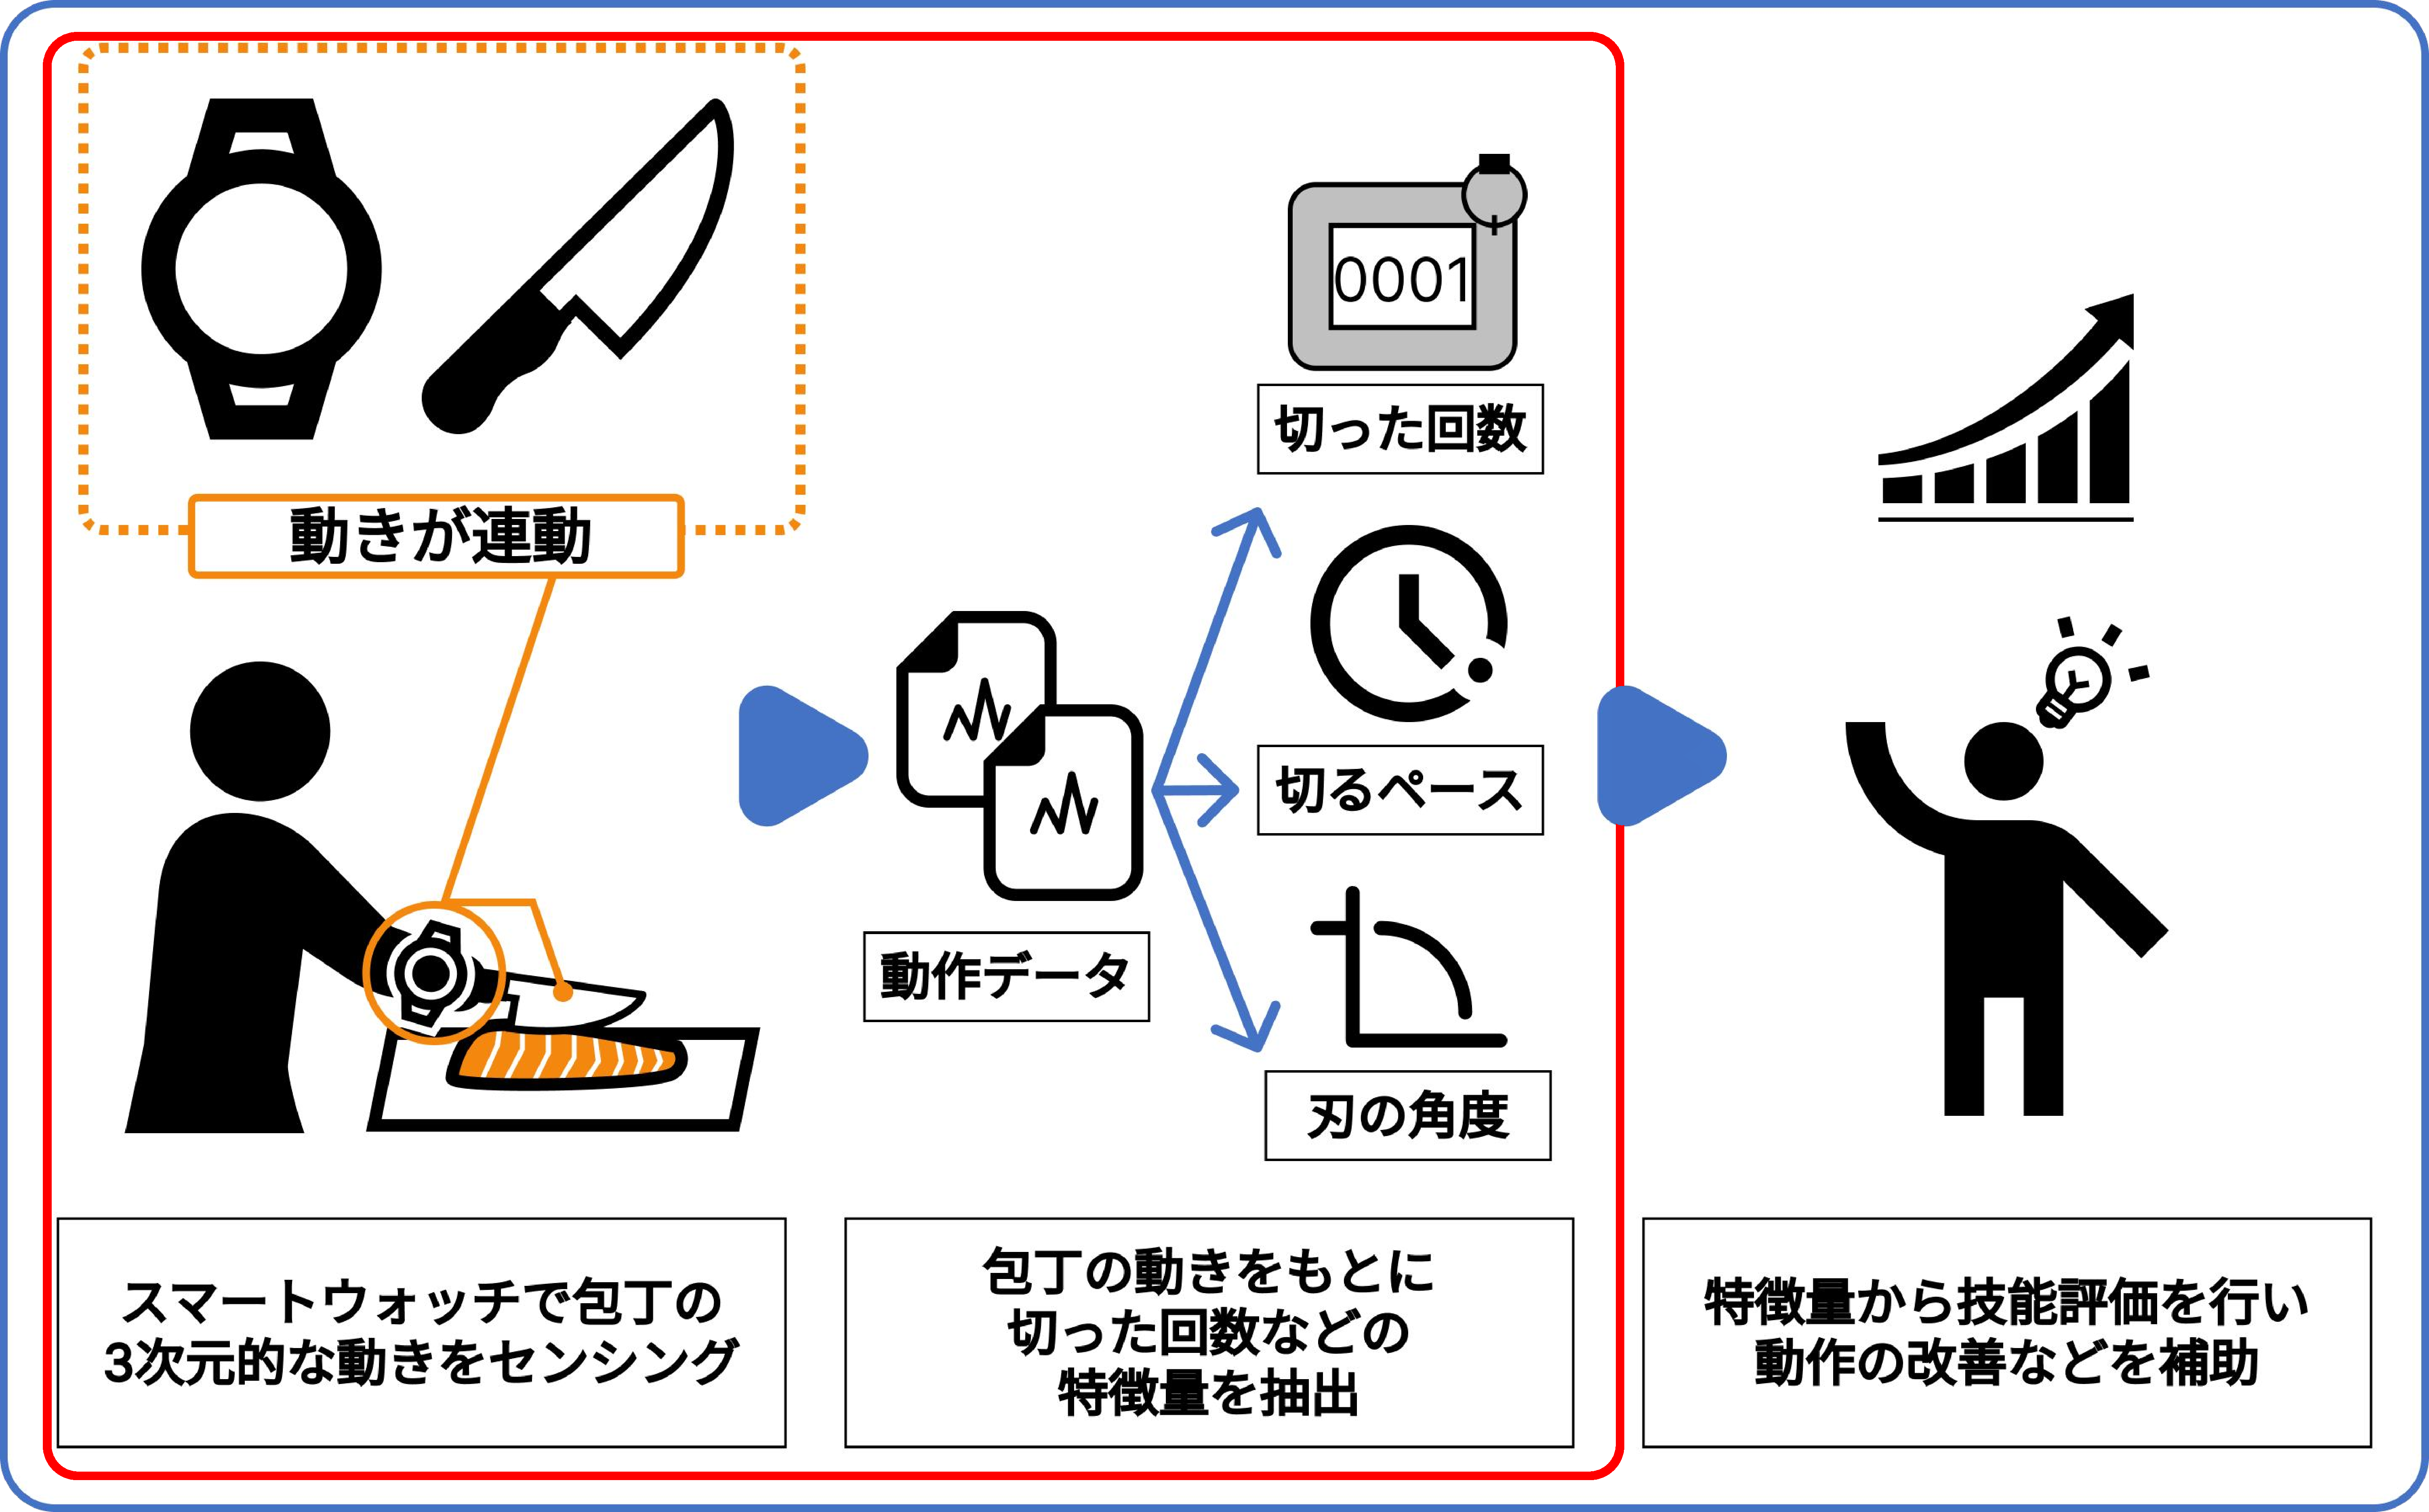
\includegraphics[width=40mm]{fig1.eps} % original

\includegraphics[width=40mm]{fig1.pdf} % suzuki
\caption{普通の図}
\label{fig:1}
\end{figure}

\begin{figure}[htb]
\centering
\subcaptionbox{多角形}{% % suzuki
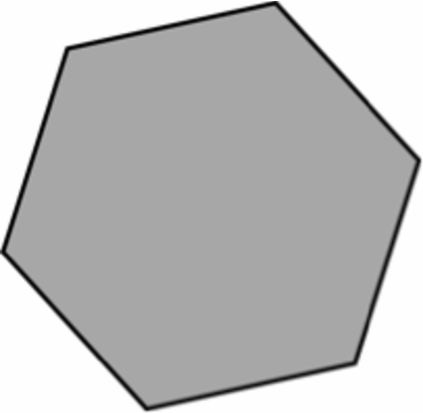
\includegraphics[height=30mm]{fig2a.pdf}}	% suzuki
\hspace{3mm}
\subcaptionbox{楕円}{%	% suzuki
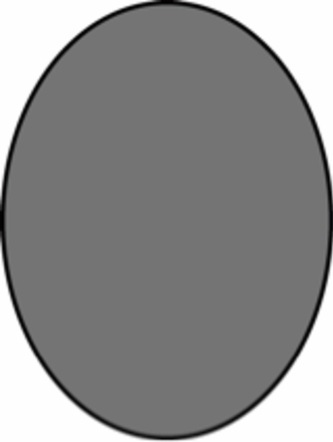
\includegraphics[height=30mm]{fig2b.pdf}}	% suzuki 
\caption{複数で構成される図}
\label{fig:2}
\end{figure}

\begin{table}[htb]
\centering
\caption{卒論卒制スケジュール}
\label{tab:sample}
\begin{tabular}{ll}\toprule
    項目     & 締切日  \\ \midrule
    レジュメ提出 & *月**日 \\ 
    卒業論文提出 & *月**日  \\ 
    発表会   & *月**日  \\ \bottomrule
\end{tabular}
\end{table}

%--------------------------------------------
\section{参考文献について}
\label{sec:reference}

必要に応じて文末に参考文献を記述する.
記述した参考文献は必ず本文中で参照する.
参考文献の書き方と本文中での参照方法を確認すること \cite{ura, tex}.

%--------------------------------------------
\section{PDFファイルの作成について}
\label{sec:pdf}

% revised by morimoto
TexShop等でPDFを作成した場合,使用する図や画像によってはファイルサイズが非常に大きくなる場合がある.
例えば「Adobe Acrobat Pro」であれば,作成したPDFファイルを「別名で保存」から「最適化されたPDF」で保存し直すことで,ファイルサイズを小さくすることができる.
解像度は少なくとも300ppiは保つようにする.

また,Mac付属のプレビューアプリでも,「書き出す」(「別名で保存」)で「Quartzフィルタ」の中の「Reduce File Size」を選択すればファイルサイズを小さくすることができる.
ただし,デフォルト設定では出力されるPDFファイル中の画像の解像度が不足する可能性があるため,フィルタ設定を自作する必要があるかもしれない.ネットで検索すれば,Quartzフィルタの作成方法はすぐに見つかる.

%--------------------------------------------
\section{まとめ}
\label{sec:conclusion}

レジュメは大量に印刷されて,同級生だけでなく後輩も見ることになる.それを踏まえて,しっかりした原稿を作成して欲しい.

%--------------------------------------------
\begin{thebibliography}{9}
\bibitem{ura}
浦正広, 遠藤守, 山田雅之, 宮崎慎也, 岩崎公弥子, 毛利勝廣, 安田孝美, ``天文教育に向けたスマートフォンの活用による対話型の星座検索モデルの提案'', 情報文化学会誌, Vol. 19, No. 2, pp.42--49, 2012.

\bibitem{tex}
奥村晴彦, 黒木祐介, ``改訂第6版 \LaTeX2$\epsilon$ 美文書作成入門'', 技術評論社, 2013.

\end{thebibliography}
\end{document}

%%% Local Variables: 
%%% mode: japanese-latex
%%% TeX-master: t
%%% End: 
